\chapter{Progettazione e Implementazione} %\label{1cap:spinta_laterale}
% [titolo ridotto se non ci dovesse stare] {titolo completo}
%

\begin{citazione}
Vero cuore della tesi, in questo capitolo vengono analizzate nel dettaglio la progettazione e l'implementazione dei due diversi moduli sviluppati. Pur condividendo le stesse finalità, i due moduli implementati presentano caratteristiche ben distinte tra loro. La scelta di tale distinzione deriva in primis dalla volontà di cimentarsi nello sviluppo di un'applicazione che consentisse a un giocatore di fronteggiare una CPU più o meno competitiva in una partita. In secundis, l'analisi delle prestazioni derivante dalla suddetta applicazione avrebbe poi spinto al confronto di diversi motori scacchistici, al fine di fornirne un'analisi delle prestazioni sempre più accurata e approfondita.
\end{citazione}

\section{Primo Modulo}
L'applicazione è stata realizzata in linguaggio Python. Come anticipato nel paragrafo precedente, l'intenzione è stata quella di sviluppare un'applicazione usabile da un utente umano per giocare una partita contro un'Intelligenza Artificiale: si è dunque ritenuta opportuna la progettazione di un'interfaccia grafica per l'interazione uomo-macchina. Attraverso la libreria \textit{pygame} è stato possibile creare l'interfaccia in modo programmatico, rappresentando le caselle con array di array di dimensione 8x8 e sfruttando semplici metodi per caricare le immagini dei pezzi precedentemente salvate nella cartella di lavoro. Inoltre, assieme ai pezzi, sono state distinte in maniera visivamente chiara e precisa le caselle chiare da quelle scure. 
\begin{figure}[!htb]
    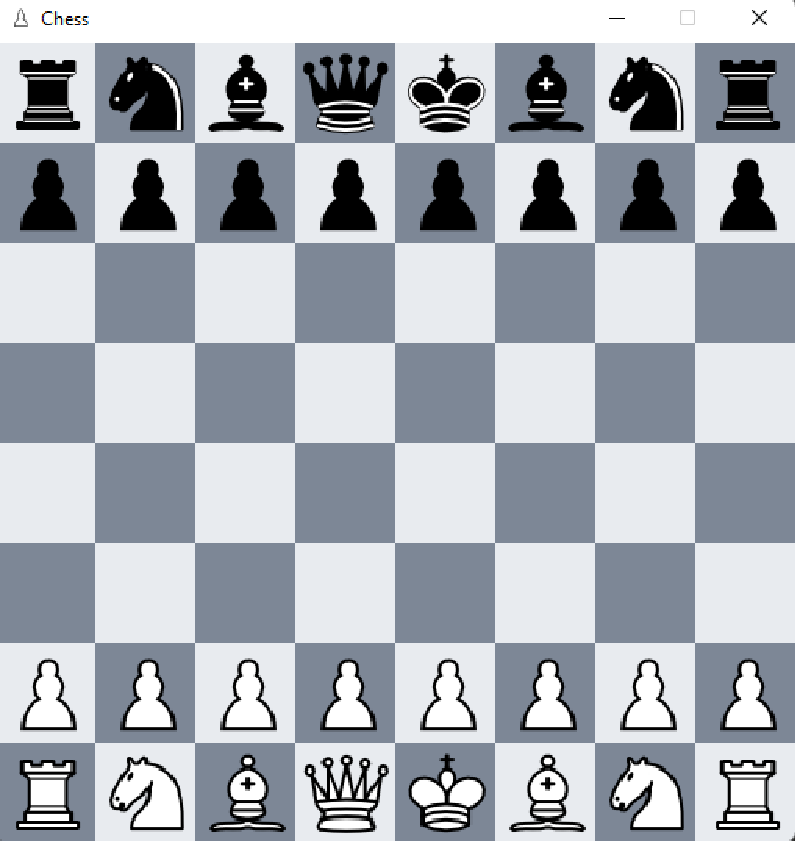
\includegraphics[width=10cm]{frontmatter/figure/scacchiera_gui.pdf}
    \centering
    \caption{Interfaccia grafica vista dall'utente}
    \label{fig:scacchiera_gui}
\end{figure}
\begin{figure}[!htb]
    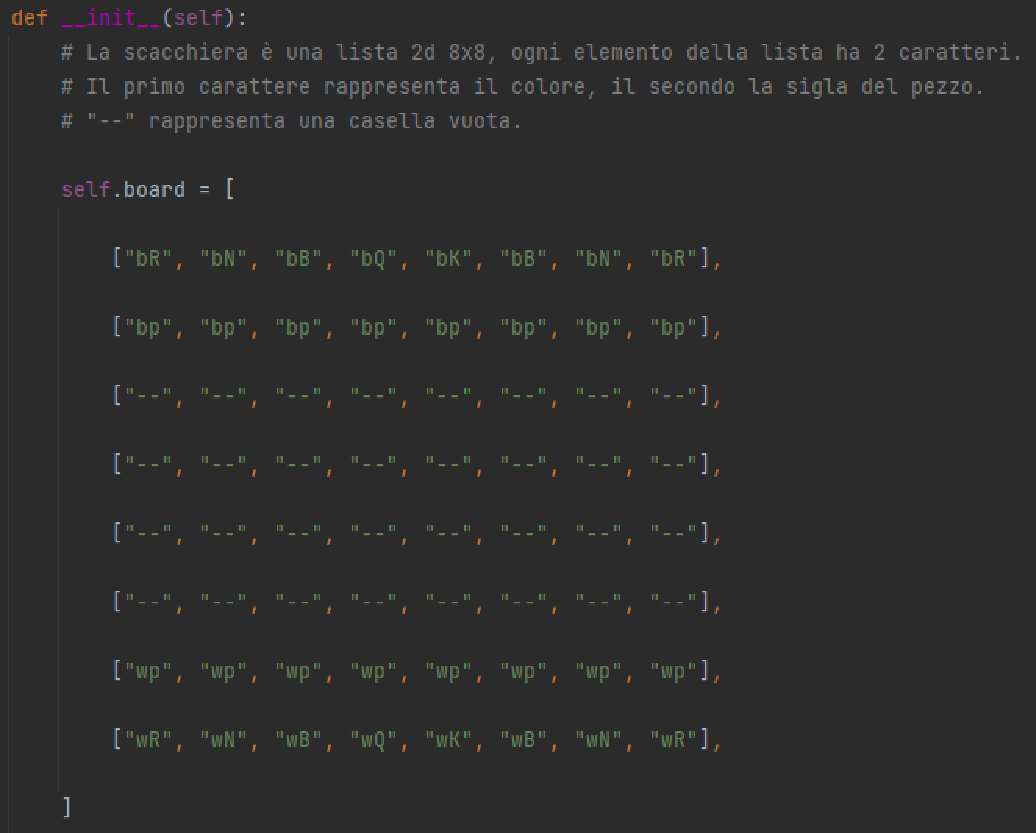
\includegraphics[width=10cm]{frontmatter/figure/rappresentazione_scacchiera.pdf}
    \centering
    \caption{Codifica della figura 3.1}
    \label{fig:rappresentazione_scacchiera}
\end{figure}
\newpage
% Per affiancare due figure
% \begin{figure}[!htb]
% \begin{minipage}[b]{7cm}
% \centering
% 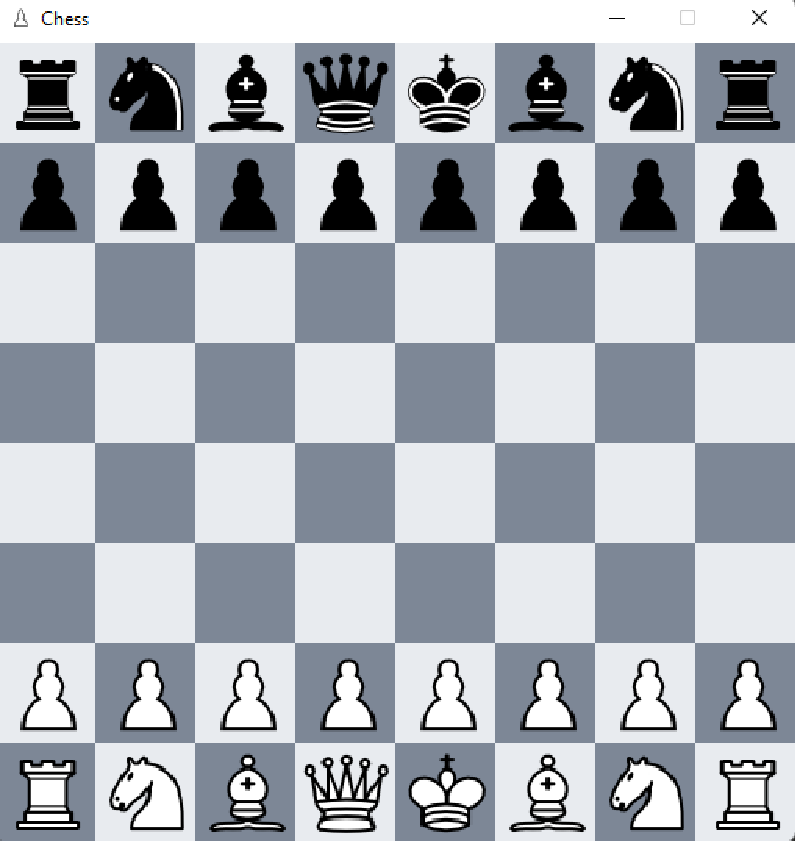
\includegraphics[width=6.5cm]{frontmatter/figure/scacchiera_gui}\\
% \caption{Interfaccia grafica vista dall'utente}
% \label{fig:scacchiera_gui}
% \end{minipage}
% \hspace{1mm}
% \begin{minipage}[b]{7cm}
% \centering
% 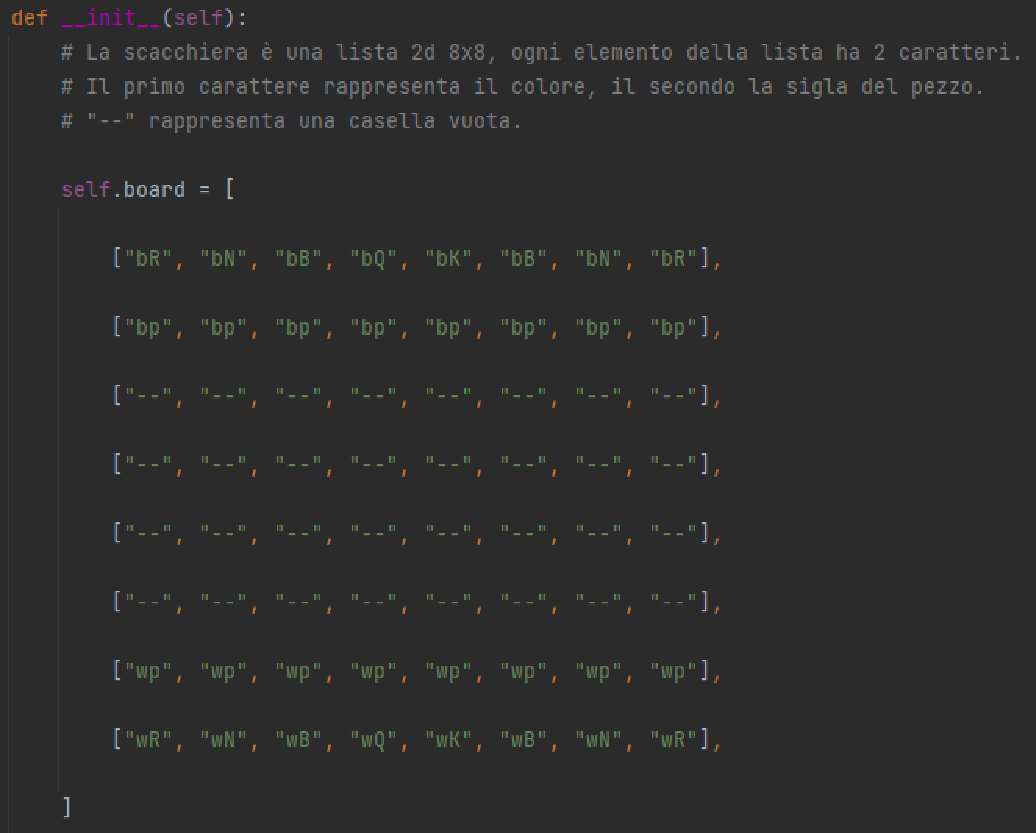
\includegraphics[width=8cm]{frontmatter/figure/rappresentazione_scacchiera}\\
% \caption{Codifica della figura 3.1}
% \label{fig:rappresentazione_scacchiera}
% \end{minipage}
% \end{figure}

A seguito della rappresentazione iniziale della scacchiera sono stati programmati i metodi che si occupano della generazione delle mosse possibili per ciascun pezzo, per impedire all'utente di effettuare mosse non legali\footnote{Nel gioco degli scacchi il pedone si muove in avanti di una casella (due per la sua prima mossa) e cattura di una casella in diagonale, la torre in orizzontale, l'alfiere in diagonale, il cavallo a L, la regina in orizzontale e in diagonale, e il re di una casella in tutte le direzioni.}. Analogamente, ad ogni mossa giocata viene effettuato un controllo nel caso in cui il re sia sotto scacco o nel caso in cui vi sia una situazione di scacco matto, dichiarando partita finita nel secondo caso.
\begin{figure}[!htb]
    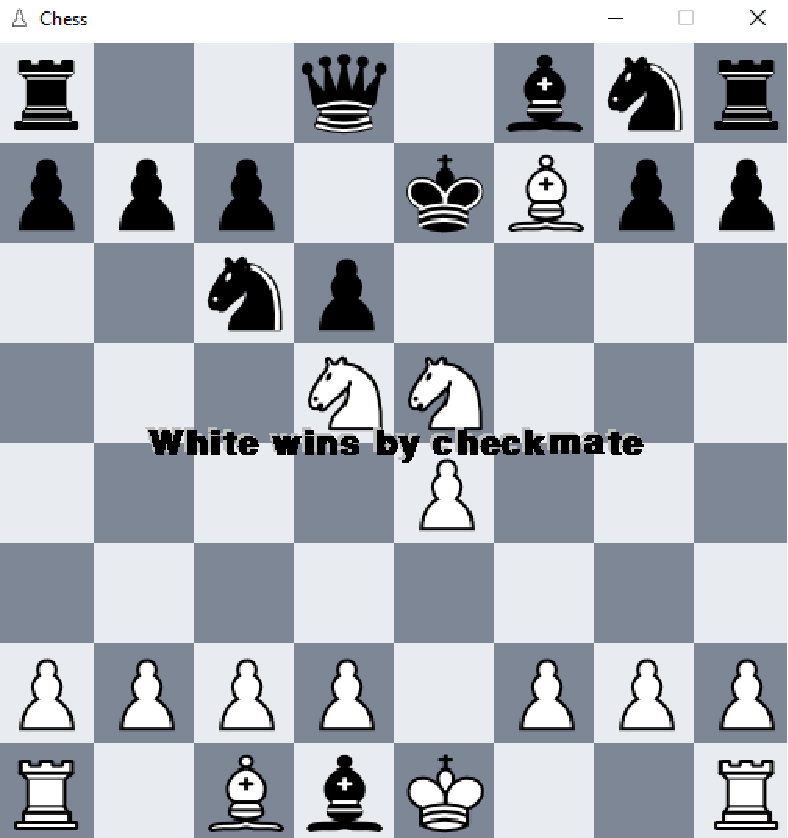
\includegraphics[width=10cm]{frontmatter/figure/checkmate.pdf}
    \centering
    \caption{Partita vinta dal bianco}
    \label{fig:checkmate}
\end{figure}


\subsection{Ricerca delle mosse legali}
Tutta la realizzazione di quanto citato sopra è stata effettuata in modo conforme alle tecniche di Intelligenza Artificiale che sono state utilizzate per la generazione delle mosse. L'obiettivo è stato quello di riprogrammare algoritmi di ricerca applicati a una rappresentazione della scacchiera che fosse familiare al programmatore, per comprenderne a fondo il funzionamento. 

\subsubsection{Algoritmo naive}
Una prima, semplice soluzione al problema è stata trovata mediante l'utilizzo di un algoritmo naive di ricerca delle mosse. Consideriamo il solito caso in cui il giocatore muove i pezzi bianchi e l'IA i pezzi neri. Dopo una qualsiasi mossa di apertura da parte del bianco, il nero ha un numero molto ristretto di opzioni tra cui scegliere: spostare uno dei pedoni in avanti di una o due caselle, o spostare un cavallo in una delle due caselle legali a inizio partita. Attraverso il metodo che ritorna la lista di mosse legali data in input una specifica situazione sulla scacchiera, l'algoritmo naive pesca a caso una delle mosse tra quelle disponibili. Chiaramente, un approccio del genere sarebbe difficilmente preso in seria considerazione nello sviluppo di un'applicazione del genere, preferendo una soluzione che tenga conto di diversi parametri (mosse storicamente giuste, valore dei pezzi, minacce possibili ai pezzi dell'avversario, trappole in apertura...). Per tale motivo, si è ritenuto necessario lo studio e l'approfondimento di altre metodologie. 

\subsubsection{Algoritmo Greedy}
Nel gioco degli scacchi è fondamentale tenere in considerazione non solo lo stato della scacchiera, ma anche il valore di ciascun pezzo (di solito, un pedone vale molto meno della regina). Sebbene sia vero che talvolta è lo stato stesso della scacchiera a determinare tale valore (a volte può essere utile sacrificare un pezzo di valore alto per vincere la partita), per convenzione si è deciso di assegnare a ciascun pezzo un valore intero di default. Questi valori sono sfruttati in un metodo di valutazione dello stato corrente della scacchiera, che indica quanto la situazione in corso sia più o meno favorevole per la vittoria.
\begin{figure}[!htb]
    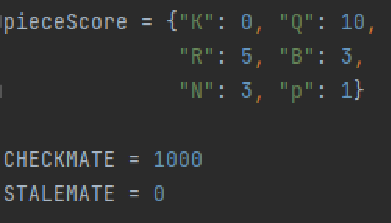
\includegraphics[width=10cm]{frontmatter/figure/valore_pezzi.pdf}
    \centering
    \caption{Oltre ai valori assegnati a ciascun pezzo si tengono in considerazione anche le situazioni di scacco matto e stallo}
    \label{fig:valore_pezzi}
\end{figure}\\

Più preciso e affidabile dell'algoritmo precedentemente considerato, l'algoritmo greedy tende più a mettere in difficoltà l'avversario piuttosto che a vincere la partita, spesso in maniera controproducente. La priorità di questa strategia è infatti quella di catturare i pezzi dell'avversario, anche a costo di mettere a rischio i propri. In ogni caso, è interessante notare come, tenendo in considerazione il valore dei pezzi, quest'algoritmo favorisca la cattura di pezzi "pesanti" piuttosto che di altri. 
\subsubsection{Algoritmo Minimax/Negamax con Potatura alfa-beta}

\subsection{Analisi delle prestazioni}
\subsubsection{Threading}
\section{Secondo Modulo}
    
\newpage
